\section{Point estimates and confidence/credible intervals}

In the previous section, we introduced the likelihood function for use in hypothesis testing and in particular rejecting hypotheses which fail some criteria based it. In this section, we'll deal with another common mode of operation for a particle physicist -- \emph{performing measurements}. In HEP, we usually report measurements of a single parameter as $X\pm\sigma_{X}$. There are a number of ways one can obtain $X$ and $\sigma_{X}$ here -- for example, it could refer to the sample mean $\bar{X}$ and standard deviation $S = \sqrt{\sum_{i}(X_{i}-\bar{X})^{2}}$ or it could refer to the moments of the distribution $f(X)$, $\mu_{1},~\sqrt{\nu_{2}}$. A very large part of what we do in HEP, is to \emph{improve on the sensitivity} of some measurement, which often involves designing experiments to measure physical quantities more precisely. Two competing experiments may claim to have measured  $X_1\pm\sigma_{X,1}$ and $X_2\pm\sigma_{X,2}$ but without knowing what they mean, we can't compare those numbers fairly. A good comparison can be made for measurements for which two properties are well understood, namely the \emph{bias} of the measured value and the \emph{coverage} of the interval. 

\subsection{Maximum likelihood estimators}
We've encountered (minimum) maximum (negative log-)likelihoods when profiling nuisance parameters. The use of maximisation/minimisation is also common in HEP when \emph{estimating} one or more parameters of interest. When choosing an estimator, a statistician will usually have in mind one or more property to be compare estimators. These can be the loss of information using a particular estimate, the variance of the estimator or even the simplicity of explaining it in a publication. What makes the \emph{maximum likelihood estimator} a good estimator is the fact that it is \emph{consistent} in the limit of large numbers, which in HEP is often the most important property. This means as the number of observations increases, the maximum likelihood estimate of a parameter converges to the real value of the parameter. Often, you'll hear particle physicists talk about the \emph{bias} of an estimator. In HEP, we often mean that either the mean ($E(\hat\theta)$) or the median of the sample distribution of $\hat{\theta}$ is equal to the true value. However, this is not quite the same thing and estimators can be unbiased but still inconsistent. For most purposes, we can however interchange the two definitions (and particle physicists will often do so as a result). We'll now show that the maximum likelihood estimate for one parameter $\theta\in\Omega$ is a consistent estimator. Note that this extends to an number of parameters, provided the likelihood function meets certain conditions (which we won't go into as in HEP it is almost always the case). 

First, recall that for multiple observations $\mathbf{X}=X_1,X_2,X_3,...,X_{N}$ of some observation, the likelihood function is defined by Eqn.~\ref{eqn:likelihoodprod}. We define the quantity $l_{N}(\theta)$, by 
\begin{equation}\label{eqn:defln}
    l_{N}(\theta) = -\frac{1}{N}\ln L(\theta) =  -\frac{1}{N}\sum_{i=1}^{N}\ln f(X_{i};\theta).
\end{equation}
Notice that minimising $l_{N}(\theta)$ is the same as maximising $L(\theta)$ since the constants have no effect on where the extreme value lies. 

By the law of large numbers, for all $\theta$, $l_{N}(\theta)\rightarrow l(\theta)$ as $N\rightarrow\infty$, where, 
\begin{equation}
    l(\theta) = E\left[-\ln(f(X;\theta))\right]_{\theta=\theta_{0}} = \int -\ln(f(X;\theta))f(X;\theta_{0})dX,
\end{equation}
and $\theta_{0}$ is the true value of $\theta$. 
The value $\theta_{0}$ is the value of $\theta$ that minimises $l(\theta)$ as can be seen from, 
\begin{eqnarray}
    l(\theta)-l(\theta_{0}) &=& \int -\ln(f(X;\theta))f(X;\theta_{0})dX- \int -\ln(f(X;\theta_{0}))f(X;\theta_{0})dX \\
     & = & \int -\ln\left(\frac{f(X;\theta)}{f(X;\theta_0)}\right)f(X;\theta_{0})dX\\
     & = & E\left[-\ln\left(\frac{f(X;\theta)}{f(X;\theta_0)}\right)\right]_{\theta=\theta_{0}} 
      \geq  -\ln\left( E \left[\frac{f(X;\theta)}{f(X;\theta_0)}\right]_{\theta=\theta_{0}}\right),
\end{eqnarray}
where in the last step, we've used Jensen’s inequality for the expectation of strictly convex functions, knowing that $-\ln(\cdot)$ is a convex function. Now we notice that, 
\begin{equation}
    \ln\left( E \left[\frac{f(X;\theta)}{f(X;\theta_0)}\right]_{\theta=\theta_{0}}\right) = \ln\left(\int \frac{f(X;\theta)}{f(X;\theta_0)}f(X;\theta_{0})dX\right) = \ln\left(\int f(X;\theta)dX\right) = \ln(1) = 0,
\end{equation}
so that, 
\begin{equation}
l(\theta)-l(\theta_{0}) \geq 0
\end{equation}
for all $\theta$ -- meaning $\theta_0$ is the value of $\theta$ that minimises $l(\theta)$. We have that for each $N$ $\hat{\theta}_{N}$ is the value of $\theta$ that minimises $l_{N}(\theta)$ and we know that $l_{N}(\theta)\rightarrow l(\theta)$ as $N\rightarrow \infty$. If the maximum likelihood estimates $\hat{\theta}$ are unique, it can be shown that $\hat{\theta}_{N}\rightarrow\theta_{0}$  as $N\rightarrow \infty$, which would prove that the maximum likelihood estimate (or minimum log-likelihood estimate) is consistent. While we won't explicitly prove this last part, it is intuitive since the sequence of likelihood functions $l_{N}$ will have minimum values that get arbitrarily close to the minimum value of $l$. Since only one value of $\theta$ minimises these functions, it makes sense that these values also get arbitrarily close to $\theta_0$.  

As we've seen (only in 1-dimension so far), obtaining the minimum log-likelihood estimates for parameters $\vec{\theta}$ can be done numerically by solving the set of equations \begin{equation}
    \nabla_{\vec{\theta}}~q(\vec{\theta}) = 0,
\end{equation} 
and we refer to the solutions as $\hat{\vec{\theta}}$. We'll take a look at a simple example to demonstrate the maximum likelihood estimator as a consistent estimator. 

\begin{tcolorbox}[colback=backblue]
\textbf{Example:} Suppose we want to estimate the two parameters $\vec{\theta} = (\mu, \sigma)$ of a normal distribution, $\phi(X;\mu,\sigma)$ given a set of observations $X_1,X_2,...,X_{N}$. The likelihood function is, 
\begin{equation}
    q(\mu,\theta) = -2\sum_{i=1}^{N}\ln\left( \frac{1}{\sigma\sqrt{2\pi}}e^{-\frac{1}{2}\left(\frac{X_{i}-\mu}{\sigma}\right)^{2}}\right) = N\ln(\sigma\sqrt{2\pi})+\sum_{i=1}^{N}\left(\frac{X_{i}-\mu}{\sigma}\right)^{2}.
\end{equation}
Suppose the true values are $\mu_{0}$ and $\sigma_{0}$. The code below shows how we can generate $N$ values of $X$ and find the maximum likelihood estimates  $\hat{\mu}$ and $\hat{\sigma}$ for increasing $N$. We'll use the \textsf{minimize} function from the \textsf{scipy.optimize} package.
\begin{lstlisting}[style = Python]
import numpy
from scipy.optimize import minimize
import matplotlib.pyplot as plt
plt.rcParams.update({'font.size': 14})

# true values
mu_0     = 4.0
sigma_0  = 2.0

# empty list of data for now
data = []

def q(params_list = []):
   mu    = params_list[0]
   sigma = params_list[1]
   N = len(data)
   sum_part = sum( [ ((x-mu)/sigma)**2 for x in data ] )
   return 2*N*numpy.log(sigma*((2*numpy.pi)**0.5)) + sum_part

# inital values for mu, sigma
init_params = [mu_0,sigma_0]
bounds  = [(-10,10),(0.01,10)]
# generate random data
steps = [5,10,20, 50, 100, 200, 500, 1000, 5000, 10000, 20000]
hat_mu = []; hat_sigma = []
for N in steps:
  data = numpy.random.normal(mu_0,sigma_0,size=N)
  mle = minimize(q,init_params,bounds=bounds)
  hat_mu.append(mle.x[0])
  hat_sigma.append(mle.x[1])

plt.plot(steps,hat_mu,color='blue',marker="o",label="$\hat{\mu}$")
plt.plot(steps,hat_sigma,color='red',marker="o",label="$\hat{\sigma}$")

plt.plot(steps,[mu_0 for s in steps],color='blue',linestyle="--")
plt.plot(steps,[sigma_0 for s in steps],color='red',linestyle="--")

plt.xlabel("N")
plt.ylabel("$\hat{\mu}$ or $\hat{\sigma}$")

plt.xscale('log')
plt.legend()
plt.show()
\end{lstlisting}
The results are shown in Figure~\ref{fig:example_mle_normal}. Clearly as $N$ increases, the maximum likelihood estimates for $\mu$ and $\sigma$ get closer to the true values.
\end{tcolorbox}
\begin{figure}[hbt!]
    \centering
    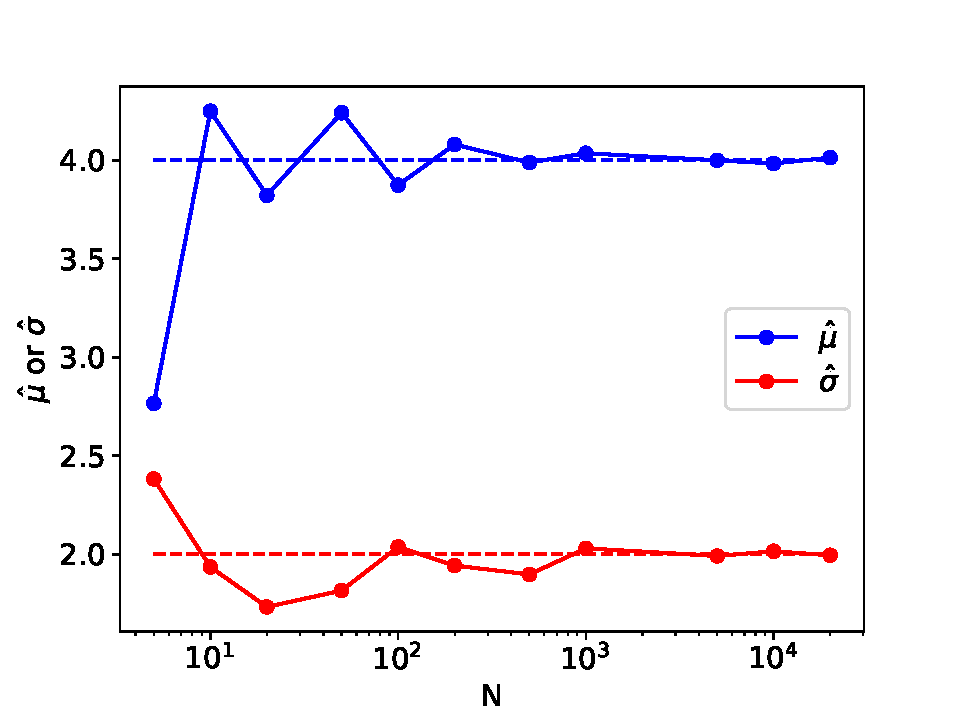
\includegraphics[width=0.8\textwidth]{figures/Intervals/Consistency_normal.pdf}
    \caption{Maximum likelihood estimates for the two parameters of a normal distribution. The likelihood is calculated from $N$ observations and the maximum likelihood estimates are determined for increasing values of $N$.}
    \label{fig:example_mle_normal}
\end{figure}
Note that in the example, we didn't need to specify whether the parameters were parameters of interest or nuisance parameters. Now we know what the $X$ refers to when a particle physicist reports a measurement as $X\pm\sigma_{X}$ -- more often than not, he/she has reported the \emph{maximum likelihood estimate} of the parameter $X$.  We are ready to discuss what the $\sigma_{X}$ means. 

\subsection{Neyman construction and frequentist confidence intervals}
The frequentist approach to reporting uncertainties on measurements is to consider the uncertainty itself as a random variable. The freqentist will report an \emph{interval} (or region in the case of more than one parameter of interest) of values of $X$ say $X_{l} \leq X \leq X_{u}$, at a specified \emph{confidence level} $(1-\alpha)$.  Knowing that $X_{l}$ and $X_u$ are random variables, the frequentist knows only that in an  ensemble of such intervals, the fraction of intervals that contain the true value $X_0$ will be $(1-\alpha)$. Note that this says nothing about whether or not a particular interval contains the true value but is only a statement about the ensemble of intervals! When a particle physicist reports s $X\pm\sigma_{X}$, the $\sigma_{X}$ might actually be written $^{+(\theta_{u}-X)}_{-(X-\theta_{l})}$ and $X_{u}$ and $X_{l}$ will usually correspond to the endpoints of the 0.683 (or 68.3\%) confidence level interval. Note that this means, if we have a composite hypothesis $H(X)$, the statement of the interval corresponds to excluding all hypotheses in the set $\left\{H(X) : X \not\in[X_{l},X_{u}]\right\}$ with an error rate of at most $\alpha$. The \emph{coverage} of a particular method to obtain those intervals is the actual fraction of intervals which contain the true value -- eg a reported 95\% confidence level interval might only cover with a fraction 0.93, meaning it \emph{under covers}. We'll see later that some methods only \emph{cover} in certain circumstances. There is a method designed to cover in all (nearly all) circumstances, known as the Neyman construction. This is explained by way of example.

\begin{tcolorbox}[colback=backblue]
\textbf{Example:} Consider the case of estimating the temperature $T$ of the fusion reactor
 at the centre of the sun by using an estimate of the solar neutrino flux $\phi$ (the test statistic) from one month's data
 from a large solar neutrino detector. Take a look at Figure~\ref{fig:neyman}. The Neyman construction uses $P(\phi|T)$ at a given value of $T$
 to choose a region in $\phi$ that constitutes $1 - \alpha$ of the probability distribution. Note that this is \emph{a} region, rather than \emph{the} region, as there are many
  possible regions containing the required fraction of outcomes. Thus the Neyman construction can be used to
 produce central regions, upper limits, lower limits, etc, simply by changing
  the ``ordering rule'' used for accumulating different test statistic values up to the required confidence level. in $\phi$  for which the fraction of outcomes in that region is a pre-determined level $1 - \alpha$, for example
  $90\%$. \\\\
  This is repeated for all values of $T$ to produce the shaded confidence band, showing the likely\footnote{We refer to the chosen values
  of $\phi$ as ``likely values'', as they are the ones selected for a particular ordering rule.}
  values of the data for any value of the parameter of interest. Then we collect one month's data, from which
  we deduce a flux $\phi_d$. The intersection of a vertical line at $\phi_d$ with the confidence band then
 gives the frequentist range for the parameter $T$, $T_{l} \leq T \leq T_{u}$, at the chosen  confidence level. 
\end{tcolorbox}
\begin{figure}[hbt!]
    \centering
    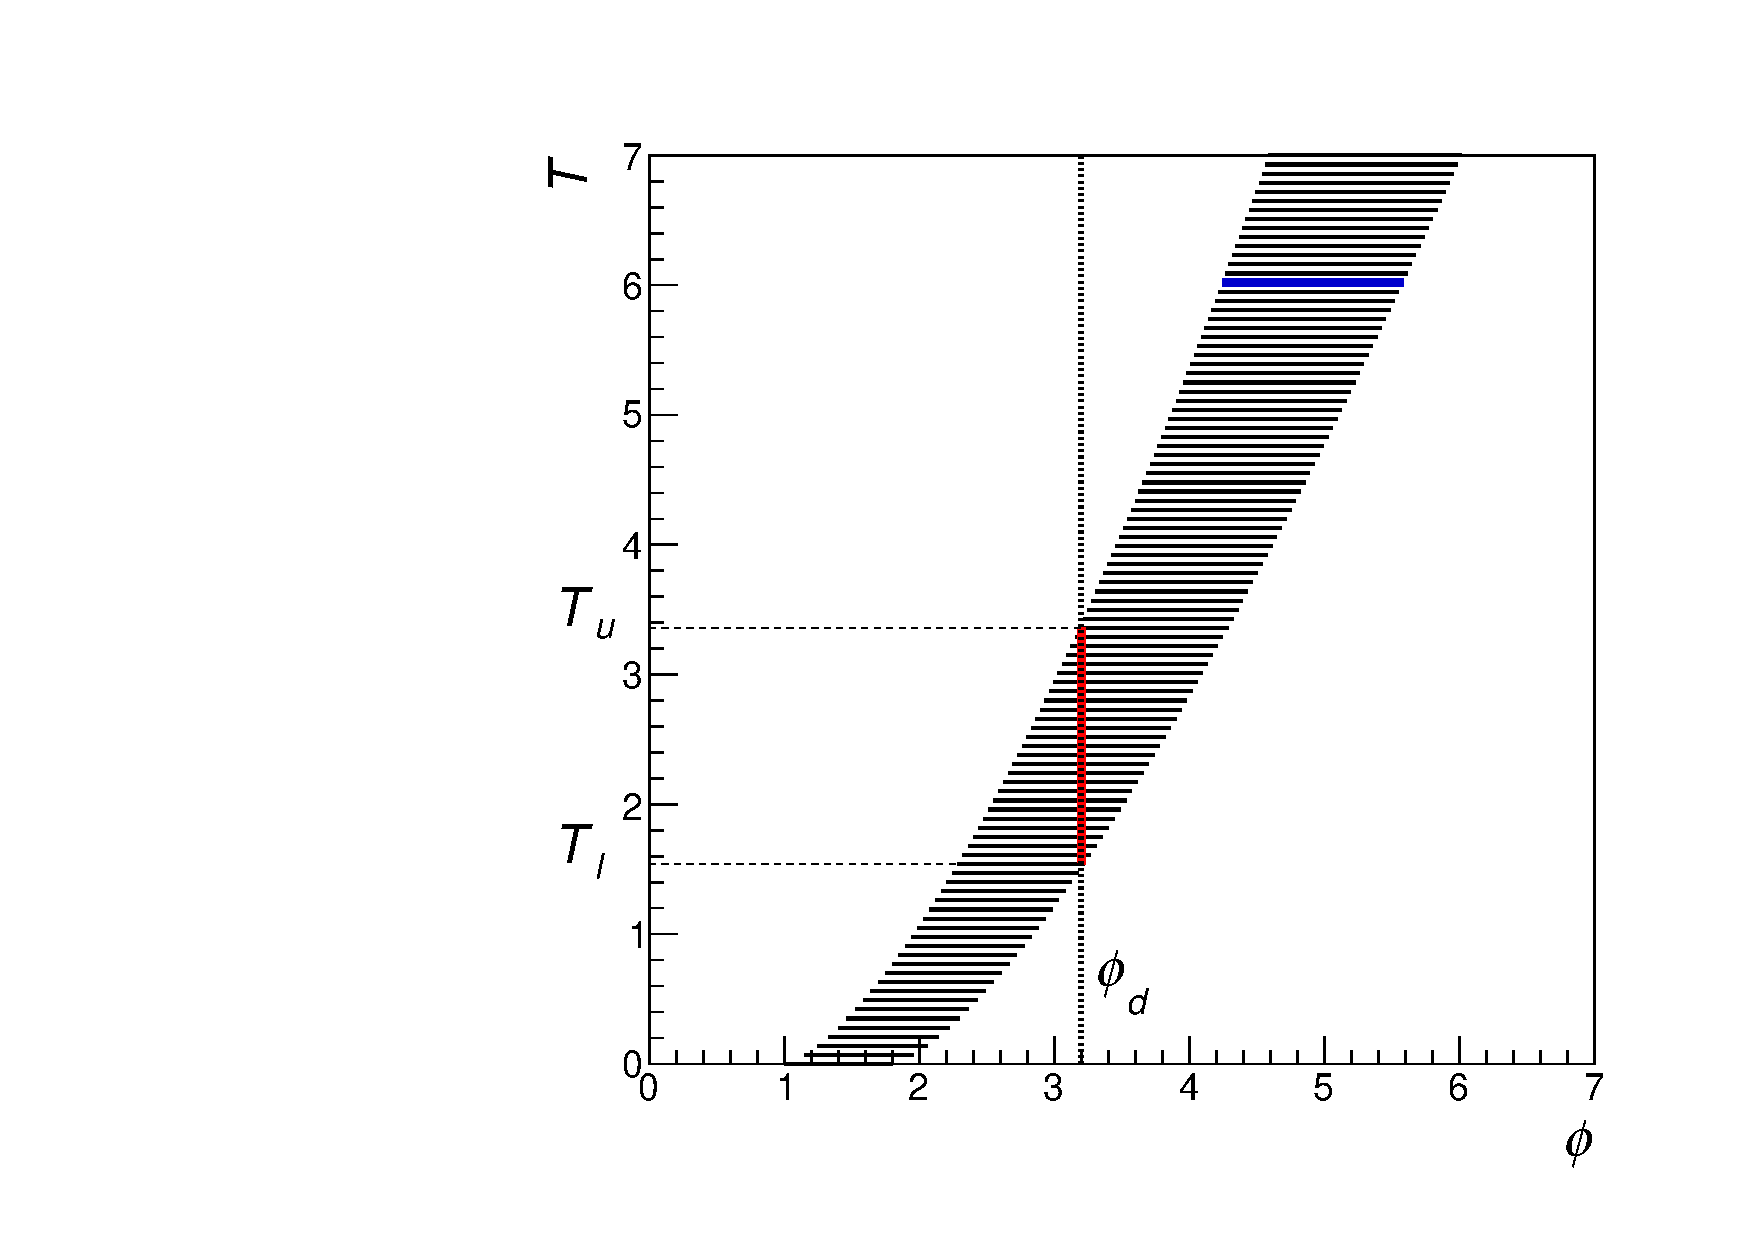
\includegraphics[width=0.6\textwidth]{figures/Intervals/neyman.pdf}
    \caption{302 The Neyman construction.  The horizontal bands gives likely values (at the 90\%
 level) of the test statistic $\phi$ (flux) for each value of the theory parameter $T$ (temperature).
 The  observed value of the test statistic $\phi_{d}$ is indicated by the vertical dotted line.
 This uses only the probability of different data, for given values of $T$;
 it does not involve probabilities of different values of $T$.
 A dotted vertical line at $\phi_{d}$ intersects
 the edges of the horizontal lines at $T_l$ and $T_u$, and these define the
 frequentist range for $T$ (indicated by the thick red vertical line). The value of $T=6$ in this case lies
 outside of the interval as the 90\% likely values of $\phi$ (indicated by the thick blue horizontal line) do not overlap with the observed value $\phi_{d}$. }
    \label{fig:neyman}
\end{figure}

In the Neyman construction, one must choose an ordering principle to select outcomes to include in the bands. In HEP (as detailed in Kendall and Stuart, and in the famous Feldman-Cousins paper \emph{"A Unified Approach to the Classical Statistical Analysis of Small Signals"}), the likelihood ratio is used to select the ``likely values'' to be included. In modern applications, this is particularly useful since it allows for a natural way to include nuisance parameters through the use of \emph{profiled} likelihoods. Moreover, often in HEP, rather than consider a sampled value $\phi$ as the test statistic and order using profile likelihood ratios, we can just use the profile likelihood ratio as the test statistic and as the ordering principle. This also very naturally extends to more than one parameter of interest. The procedure is as follows;
\begin{itemize}
    \item Define the test statistic using the profiled likelihood function $L$ as, 
    \begin{eqnarray}
        \zeta_{\mu} &= & \begin{cases}
               q(\mu,\hat{\eta}_{\mu})-q(\hat{\mu},\hat{\eta})    & \hat{\mu} \in \Omega \\
               q(\mu,\hat{\eta}_{\mu})-q(\hat{\mu}_{\Omega},\hat{\eta}_{\hat{\mu}_{\Omega}})            & \mathrm{else,}
                \end{cases}
    \end{eqnarray}
    where as usual $\mu$ are the parameters of interest bounded to $\mu\in\Omega$ and $\eta$ are the nuisance parameters, and $\hat{\mu}_{\Omega}$ means the value of $\mu$ that satisfies $\mathrm{max}\left\{q(\mu,\hat{\eta}_{\mu}):\mu\in\Omega\right\}$. 
    In the case of only one parameter of interest, the boundary condition can be expressed as $\mu\in[\mu_{a},\mu_{b}]$. 
    \item For each value of $\mu\in\Omega$ (representing the hypothesis $H(\mu)$), calculate $\zeta_{\mu}^{\mathrm{obs}}$ for the observed data and generate toy data (including for the constraint terms of any nuisance parameters, using their profiled values to define their probability density functions), to calculate the distribution $f(\zeta_{\mu}|H(\mu))$. 
    \item Choose a confidence level $(1-\alpha)$ and select the values of $\mu$ for which, 
    \begin{equation}
        p_{\mu}= \int_{\zeta_{\mu}^{\mathrm{obs}}}^{+\infty} f(\zeta_{\mu}|H(\mu)) d\zeta_{\mu} \geq \alpha.
    \end{equation}
    The union of all of these values forms the $100\times(1-\alpha)\%$ confidence region (interval for 1 parameter). Note that the ordering principle that we've used to calculate $p_{\mu}$ is the same as the Feldman-Cousins ordering rule (in the case of no nuisance parameters) and Kendall and Stuart (with nuisance parameters).  
\end{itemize}

\begin{tcolorbox}[colback=backblue]
\textbf{Example:} Let's go back to our example with the simple counting experiment, this time we'll determine the 68\% confidence interval on the parameter $\mu$, and keep the boundary on the parameter $\mu\geq0$, or in other words $\Omega = [0,+\infty)]$. A lot of the code can be repeated from when we were calculating the upper limit, however we need to change our test statistic as follows,
\begin{lstlisting}[style = Python]
# calculate test statistic
def zetamu(np,eta_p,mu):
  q_value        = q(mu,profiled_eta(mu,np,eta_p),np,eta_p)
  q_min,mu_min   = global_min(np,eta_p)
  if mu_min < 0 : return q_value-q(0,profiled_eta(0,np,eta_p),np,eta_p)
  else          : return q_value-q_min
\end{lstlisting}
and follow the procedure above. We loop over different values of $\mu$ and store the distributions using something like the code below, 
\begin{lstlisting}[style = Python]
import numpy
from model import *
from scipy.optimize import minimize
  
def global_min(np,eta_p):
  init_params = [0.1,-3.]
  bounds = [(-1,50),(-5,5)]
  # note q_constrained is the same function as q but 
  # with keyword arguments for the minimize function
  mle = minimize(q_unconstrained,\
        init_params,args=[np,eta_p],bounds=bounds)
  return mle.fun,mle.x[0]
  
mu_range   = numpy.arange(0,8,0.2)
zeta_range = numpy.arange(0,10,0.1)

# generate distribution f(zeta_mu) and find zeta_mu^68
def histo_zetamu(mu,zeta_obs):
  eta_profiled = profiled_eta(mu,n,0)
  ntoys = 10000
  toy_n   = numpy.random.poisson(lamb(mu,eta_profiled),size=ntoys)
  toy_eta = numpy.random.normal(eta_profiled,1,size=ntoys)
  zetamu_dist = [zetamu(np,eta_p,mu) for np,eta_p in zip(toy_n,toy_eta)]
  zetamu_dist.sort() ; zeta_68 = zetamu_dist[int(ntoys*0.68)]
  return zetamu_dist, zeta_68
 
# store the results as we go through the loop
zeta_obs_vals, zeta_68_vals = [], []
mu_interval, densities = [], []

# loop over mu values and see which ones pass the criteria
for mu_test in mu_range:
  zeta_obs = zetamu(n,0,mu_test)
  zetamu_toys,zeta_68 = histo_zetamu(mu_test,zeta_obs)
  density_vals = plt.hist(zetamu_toys,density=True,bins=zeta_range)
  densities.append(density_vals[0])
  zeta_68_vals.append(zeta_68)
  zeta_obs_vals.append(zeta_obs)
  if zeta_obs < zeta_68 : mu_interval.append(mu_test)
\end{lstlisting}

Figure~\ref{fig:neyman_counting} shows the distribution $f(\zeta_{\mu}|H(\mu))$ for fixed values of $\mu$. Also shown is the \emph{observed value} $\zeta^\mathrm{obs}_{\mu}$ -- unlike the solar temperature example, this is not a single number but of course depends on $\mu$. Finally, also plotted is the value of $\zeta_{\mu}$ (called $\zeta_{\mu}^{68}$) which is larger than 68\% of the toys in the distribution. This means that the values of $\mu$ to be included in the interval are those for which $\zeta^\mathrm{obs}_{\mu}< \zeta_{\mu}^{68}$. Keeping track of which $\mu$ values meet the criteria, the interval is be $0.50\leq\mu\leq6.20$. Note that we also know the maximum likelihood estimate of $\mu$ since its (by definition) the value of $\mu$ for which $\zeta_{\mu}=0$. Finally then we can say that our frequentist measurement is $\mu=2.22^{+3.98}_{-1.72}$.
%Note, to simplify things, I'm also going to stick to using the \textsf{scipy.optimize.minimize} function in my code.  
\end{tcolorbox}
\begin{figure}[hbt!]
    \centering
    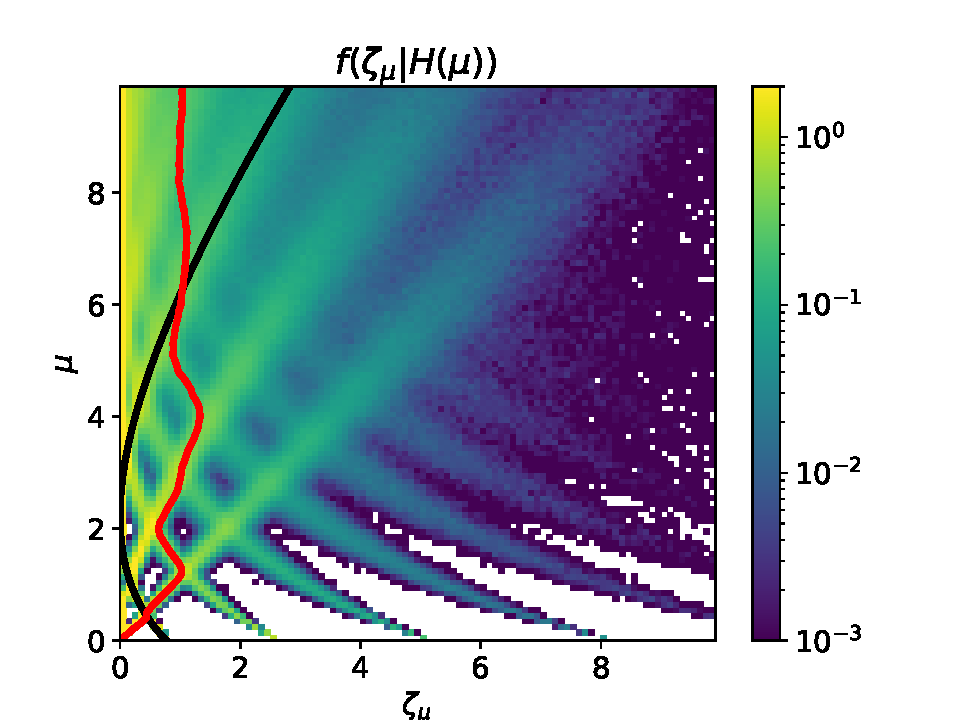
\includegraphics[width=\textwidth]{figures/Intervals/frequentist_interval.pdf}
    \caption{Distributions $f(\zeta_\mu|H(\mu))$ for different values of $\mu$ are shown by the color scale. The white regions show where there are no entries, highlighting the discrete nature of the Poisson probability distribution. The black like shows the observed values $\zeta_\mu^{\mathrm{obs}}$ and the red line shows $\zeta_{\mu}^{68}$ -- the value that 68\% of the distribution is smaller than. The values of $\mu$ for which $\zeta_\mu^{\mathrm{obs}} < \zeta_{\mu}^{68}$ form the 68\% confidence interval. }
    \label{fig:neyman_counting}
\end{figure}
In the counting experiment example, we saw that the region of $\zeta_{\mu}$ which contained 68\% of the toy data changed as a function of $\mu$, jumping around when $\mu\sim 0$. This is due to the discrete nature of the Poisson probability distribution and the effects of the boundary at $\mu=0$. However, for larger values of $\mu$, we see that this value seems to stay the same and becomes \emph{independent} of $\mu$. This is not so surprising given the law of large numbers since we know that as $\lambda\rightarrow \infty$, the Poisson distribution tends to a normal one. Furthermore, for \emph{any} likelihood function, the central limit theorem tells us that the likelihood estimator (which is a random value) should be distributed as a normal distribution. In the limit of large numbers then, there is no need to determine the $\zeta_{\mu}^{68}$ values using toys or even to determine the distribution at all with toys -- this is a convenient result (theorem) by \emph{Wilks'}. 

\subsection{Wilks' theorem and the MINOS method}
Wilks' theorem provides a very powerful result that allows us to calculate the distribution of $\zeta_{\mu}$, under certain conditions, in the limit of a large sample size. The most important of these conditions that particle physicists sometimes ignore is that the maximum likelihood estimate must not be at or beyond a boundary of the parameter space. In our counting experiment, this means that introducing the condition $\mu>0$, will have implications when the maximum likelihood estimate is close to 0. There are other conditions, but in HEP these are almost always satisfied so there's no need to cover them. 

Let's start with the simplest case where we have a single parameter of interest $\theta$ with no nuisance parameters. As usual, for $N$ observations of a random variable $X\sim f(X;\theta)$, we define, 
\begin{equation}
    \zeta_{N,\theta} = q_{N}(\theta)-q_{N}(\hat{\theta}) = -2\sum_{i=1}^{N}\ln f(X_{i};\theta) + 2\sum_{i=1}^{N}\ln f(X_{i};\hat{\theta}) .
\end{equation}
Providing that the derivatives of $f$ exist, we can Taylor expand the first derivative of $q_N$ to approximate the value at $\hat{\theta}$, 
\begin{equation}
   0= \frac{dq_{N}}{d\theta}\bigg|_{\theta=\hat{\theta}} = q_{N}'(\hat{\theta})  = q_{N}'(\theta)+q_{N}''(\theta) (\hat{\theta}-\theta),
\end{equation}
where the first equality is due to the fact that $\hat\theta$ is the value of $\theta$ that maximises the likelihood function $q_{N}$. We can re-write the equation as, 
\begin{equation}\label{eqn:randvarwt}
    (\hat{\theta}-\theta)\sqrt{q''_{N}(\theta)} = -\frac{q'_{N}(\theta)}{\sqrt{q''_{N}(\theta)}},
\end{equation}
which looks like an odd thing to do but it will be useful. Looking at the numerator on the RHS, we have, 
\begin{equation}
    -q'_{N}(\theta) = \frac{d}{d\theta}\sum_{i=1}^{N}2\ln f(X_{i};\theta)= \sum_{i=1}^{N} 2\frac{d}{d\theta}\left(\ln f(X_{i};\theta)\right).
\end{equation}
Now let's define the random variable $u=2\dfrac{d}{d\theta}\ln f(X|\theta)$, then we have that $-q'_{N}(\theta)$ looks like a sample mean of this random variable. In fact $-q'_{N}(\theta)=N\bar{u}$, where $\bar{u}$ is the sample mean of $u$. The expectation of $u$ can be found by considering that for any $\theta$,
\begin{eqnarray}
    1 &=& \int f(X;\theta)dX,                      \\
\end{eqnarray}
and therefore, taking derivatives,
\begin{eqnarray}
    0 &=& \frac{d}{d\theta} \int f(X;\theta)dX = \int \frac{d}{d\theta}  f(X;\theta)dX = \int \frac{d}{d\theta} \left(\ln f(X;\theta)\right)\cdot f(X;\theta)dX  \\ 
      &=& E\left[\frac{d}{d\theta}\ln f(X;\theta)\right]_{\theta} = \frac{1}{2}E\left[u\right]_{\theta},  
\end{eqnarray}
and hence the expectation of $u$ under $f(X;\theta)$ is 0. 
We can start to form a quantity $T_{N}$, given by, 
\begin{equation}
    T_{N,\theta} = \frac{N\bar{u} - NE[u]_{\theta}}{\sqrt{N\cdot V(u)_{\theta}}}
\end{equation}
We want to see what happens in the limit of $N\rightarrow\infty$, to the quantity $\sqrt{q''(\theta)}$. If its proportional to $\sqrt{N\cdot V(u)_{\theta}}$, then we have, by the central limit theorem, that $T_{\theta}$ (the limit of $T_{N,\theta}$) is distributed as $T_{\theta}\sim\phi(T_{\theta};0,1)$.

Let's take a look at $V(u)_{\theta}$. We have by definition that, \begin{eqnarray}
    V(u)_{\theta} & = &  E\left[(u-E[u]_{\theta})^{2}\right]_{\theta} = E\left[(u)^{2}\right]_{\theta} \\
     & = & 4\int \left(\frac{d}{d\theta}\ln f(X;\theta)\right)^{2}f(X;\theta)dX.
\end{eqnarray}
Recall again that, 
\begin{eqnarray}
    1 & = & \int f(X;\theta)dX
\end{eqnarray}
and differentiating twice we have, 
\begin{eqnarray}
    0 & = & \int \frac{d}{d\theta}\left(\frac{d}{d\theta}\ln f(x;\theta)\cdot f(X;\theta)\right)dX \\
     & = & \int \frac{d^2}{d\theta^2}\ln f(X;\theta) \cdot f(X;\theta)dX +  \int \frac{d}{d\theta}\ln f(X;\theta) \cdot \frac{d}{d\theta}f(X;\theta)dX  \\
     & = & \int \frac{d^2}{d\theta^2}\ln f(X;\theta) \cdot f(X;\theta)dX +  \int \frac{d}{d\theta}\ln f(X;\theta) \cdot \frac{d}{d\theta}\ln f(X;\theta)\cdot f(X;\theta) dX\\ 
     & = & \int \frac{d^2}{d\theta^2}\ln f(X;\theta) \cdot f(X;\theta)dX +  \int \left(\frac{d}{d\theta}\ln f(X;\theta) \right)^{2} f(X;\theta) dX \\
     & = & \int \frac{d^2}{d\theta^2}\ln f(X;\theta) \cdot f(X;\theta)dX +  \frac{1}{4}V(u)_{\theta}, 
\end{eqnarray}
so that, 
\begin{eqnarray}
\frac{1}{4}V(u)_{\theta} = - \int \frac{d^2}{d\theta^2}\ln f(X;\theta) \cdot f(X;\theta)dX = - E\left[\frac{d^{2}}{d\theta^{2}}\ln f(X;\theta)\right]_{\theta}.
\end{eqnarray}
But remember that $q''_{N}(\theta) = -2 \sum_{i=1}^{N} \dfrac{d^2}{d\theta^2}\ln f(X;\theta)$. By the law of large numbers, we must have that $\dfrac{-q''_{N}(\theta)}{N}\rightarrow 2E\left[\dfrac{d^2}{d\theta^2}\ln f(X;\theta)\right]_{\theta}$ as $N\rightarrow \infty$. But this is just $-\dfrac{1}{2}V(u)_{\theta}$! So then we have $\dfrac{q''_{N}(\theta)}{N}\rightarrow  \dfrac{1}{2}V(u)_{\theta}$.
Now (in a rather hand-wavy fashion), we can say that,
\begin{eqnarray}\label{eqn:part1}
  \frac{1}{\sqrt{2}}(\hat{\theta}-\theta)\sqrt{q''_{N}(\theta)}  = -\frac{q'_{N}(\theta)}{\sqrt{2 q''_{N}(\theta)}} \rightarrow 
\frac{q'_{N}(\theta)}{\sqrt{N\cdot V(u)_{\theta} }} = \frac{N\bar{u}-NE[u]_{\theta}}{\sqrt{N\cdot V(u)_{\theta} }} = T_{N,\theta} \rightarrow T_{\theta}\sim\phi(T_{\theta};0,1).
\end{eqnarray}
We've been a bit careless here since the numerator converges in distribution and the denominator converges in probability, and we've performed the two limits separately. However, but there is a theorem (which we won't go into) for ratios of such random variables, numerator converging in distribution and denominator in probability, due to Slutsky which yields the same result so in the end its ok.  

Let's go back to the definition of $\zeta_{N,\theta}.$ Again, we take a Taylor expansion, this time of the function $q_{N}(\theta)$,
\begin{equation}\label{eqn:taylor_exp_qN}
    q_{N}(\theta) = q(\hat\theta) + \cancelto{0}{q'_{N}(\hat{\theta})}(\theta-\hat{\theta}) + \frac{1}{2}q''_{N}(\hat\theta)(\theta-\hat{\theta})^2,
\end{equation}
and so, 
\begin{equation}\label{eqn:part2}
    \zeta_{N,\theta} =  \frac{1}{2}q''_{N}(\hat\theta)(\theta-\hat{\theta})^2 = \left( \frac{1}{\sqrt{2}}(\hat{\theta}-{\theta})\sqrt{q''_{N}(\hat\theta)}\right)^2. 
\end{equation}
Now the term inside the square on the RHS of Eqn~\ref{eqn:part2} is the same as in the LHS of Eqn.~\ref{eqn:part1}, except for the value of $\theta$ at which the second derivative is evaluated. However, since the maximum likelihood estimate is \emph{consistent}, $\hat\theta\rightarrow \theta_{0}$ as $N\rightarrow \infty$. So in the limit $N\rightarrow \infty$, we replace $\theta$ with $\theta_{0}$, and study the distribution of $\zeta_{\theta}$ for the true value of $\theta=\theta_{0}$. In this limit we can then equate the LHS of Eqn.~\ref{eqn:part1} with the term inside the square, so that, 
\begin{equation}
    \zeta_{N,\theta_0} = (T_{N,\theta_{0}})^2.
\end{equation}
But we know that $T_{N,\theta_0}$ is distributed as a unit normal $\phi(T;0,1)$ under the hypothesis $H(\theta_0)$ \emph{for any value of $\theta$} as $N\rightarrow \infty$ so we can also figure out the distribution of $(T_{N,\theta_{0}})^2$. This distribution is known as a $\chi^{2}$ -- a \emph{chi-square} distribution with 1 degree of freedom. It has the probability density function, 
\begin{equation}
    \chi^{2}(X;1) = \frac{1}{\sqrt{2\pi X}}e^{-\frac{X}{2}}.
\end{equation}
This is the result of Wilks' theorem for one parameter. In general, Wilks' theorem gives us the result for any number of degrees of freedom. The result is that for a log-likelihood difference with $n$ parameters $\theta_{1},\theta_{2},...,\theta_{n}$, the test statistic $\zeta_{\theta_{1},...,\theta_{n}}$ will be distributed under $H(\theta_{1},...,\theta_{n})$ (the null hypothesis) as, 
\begin{equation}
  f(\zeta_{\theta_{1},...,\theta_{n}}|H(\theta_{1},...,\theta_{n})) = \chi^{2}(\zeta_{\theta_{1},...,\theta_{n}};n),
\end{equation}
where $\chi^{2}(\cdot;n)$ is the chi-square distribution with $n$ degrees of freedom, in the limit of large sample sizes. 
If we know the distribution of $\zeta$, then we can calculate $p_{\theta}$ for any value of $\zeta_{\theta}$ by looking up the cumulative distribution function of the $\chi^2$ functions. Moreover, the value of $\zeta^{68}_\theta$ (and any quantile, not just the 68\% one) is independent of $\theta$!. Any one of your favourite statistics programming languages will be able to calculate this for you, for example in python, we can use the \textsf{scipy.stats.chi2} class and use the \textsf{chi2.cdf} function. Figure~\ref{fig:chisquare} shows the probability density and cumulative density functions for the $\chi^{2}$ with increasing numbers of degrees of freedom. Using the cumulative distribution, it is possible to read off $p-$values or the value of $X$ that would contain some percentage of the distribution. 
\begin{figure}[hbt!]
    \centering
    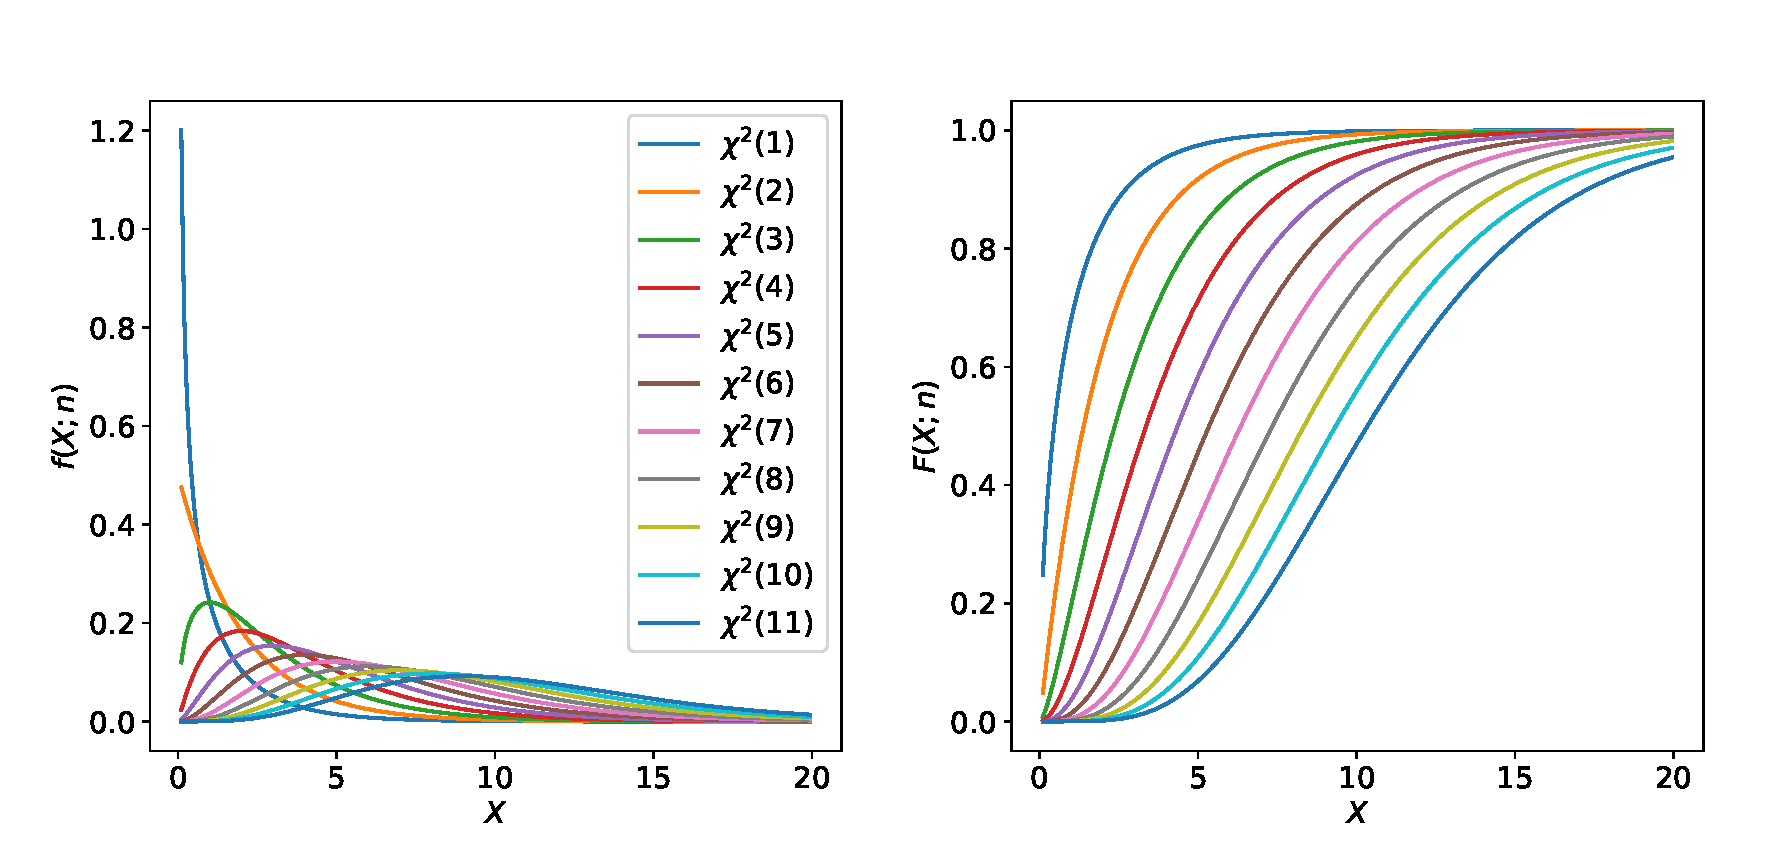
\includegraphics[width=\textwidth]{figures/Intervals/chi2dists.pdf}
    \caption{Probability density (left) and cumulative density (right) functions for the $\chi^{2}$ with increasing numbers of degrees of freedom.}
    \label{fig:chisquare}
\end{figure}
Calculating intervals or confidence regions for parameters becomes straightforward since for each value, we know the distribution of $\zeta_{\theta}$ under the hypothesis $H(\theta)$ simply by knowing the dimension of $\theta$ and calculating $\zeta_{\theta}^{\mathrm{obs}}$. The $(1-\alpha)$ confidence region in $n-$dimensions is determined by the values of $\theta$ for which,
\begin{equation}
    \zeta_{\theta}^{\mathrm{obs}}=q(\theta)-q(\hat{\theta})=
    \Delta q(\theta) \leq Q
\end{equation}
where $\int_{Q}^{+\infty} \chi^{2}(\zeta_{\theta};n)d\zeta_{\theta} = \alpha$. For example, if $n=1$ and $(1-\alpha)=0.683$, then  $Q=1$, while if $n=1$ and $(1-\alpha)=0.954$, then $Q=4$. In our goodness of fit test, we could have used this result to calculate the $p-$value and our number of degrees of freedom would be the number of bins. 

Let's look at an example of trying to measure two signal rates over a falling background distribution, using a binned likelihood. We'll include nuisance parameters, but remember that we don't include them in the definition of the test-statistic -- they are profiled.  

\begin{tcolorbox}[colback=backblue]
\textbf{Example:} We have an analysis in which the number of events in bins of a distribution is counted. There is a background process and two signal processes with signal strength modifiers $\mu_1$ and $\mu_2$, with no restrictions on their range. Our log-likelihood function for this will be, 
\begin{equation}
    q(\mu_1,\mu_2,\eta) = -2 \left(\sum_{i} n\ln{\lambda_{i}}- \lambda_{i} \right) + \eta^{2},
\end{equation}
where $i$ runs over the bins, $\lambda_{i}=\mu_{1}s_{i,1}+\mu_{2}s_{i,2}+b_{i}(1+k_{i})^{\eta}$,
and $\eta$ is a nuisance parameter which can change the slope of the background (due to the $\kappa_{i}$ being different for each bin. 
The model can is defined using the snippet below, 
\begin{lstlisting}[style = Python]
signal1_counts=[0,0,0,0.5,1,2,3,4,5,4.5,4.0,3.5,3.0,2.5,2,\ 
    1.5,1,0.5,0,0,0,0,0,0,0]
    
signal2_counts=[0,0,1,2,3,4,5,6,5,3,1,0,0,0,0,0,\ 
    0,0,0,0,0,0,0,0,0]
    
background_counts=[60*numpy.exp(-0.1*i) \
    for i in range(len(signal1_counts))]
    
bkg_uncert=[0.3,0.3,0.3,0.2,0.2,0.2,0.2,0.2,0.2,0.1,0.1,0.1,\
    0.1,0.1,0.1,0.1,0.1,0.05, 0.05,0.05,0.05,0.02,0.02,0.02,0.02]
    
nbins = len(signal1_counts)

def lamb(i,mu1,mu2,eta):
  s1 = signal1_counts[i]
  s2 = signal2_counts[i]
  b = background_counts[i]
  k = bkg_uncert[i]
  return mu1*s1+mu2*s2+b*(1+k)**eta

data=[65,45,47,37,37,40,42,36,34,36,22,23,23,18,\ 
    17,13,12,12,11,12,6,6,6,9,4]
\end{lstlisting}
Figure~\ref{fig:example_binneddata} shows the background and signal distributions at the global minimum $(\hat{\mu}_{1},\hat{\mu}_{2},\hat{\eta})$. The data is shown on top with each data point indicating the standard deviation of a Poisson distribution with the same mean as the observed data in that bin. We scan the value of, 
\begin{equation}
    \Delta q(\mu_1,\mu_2) =  q(\mu_1,\mu_2,\hat{\eta}_{\mu_1,\mu_2}) - q(\hat{\mu}_1,\hat{\mu}_2,\hat{\eta}).
\end{equation}
Figure~\ref{fig:example_binnedlh} shows the value using a color scale. Using Wilks' theorem, the 68.3\% and 95.4\% confidence regions are the regions for which $ \Delta q(\mu_1,\mu_2) < 2.3$ and  $ \Delta q(\mu_1,\mu_2) < 5.99$ respectively, as indicated by the contours. If we are interested in only the first parameter, $\mu_1$, then we can use the function,  
\begin{equation}
    \Delta q(\mu_1) =  q(\mu_1,\hat{\mu}_{2,mu_{1}},\hat{\eta}_{\mu_1}) - q(\hat{\mu}_1,\hat{\mu}_2,\hat{\eta}).
\end{equation} 
The 68.3\% and 95.4\% intervals are found as the region for which  $\Delta q(\mu_1)<1$ and $\Delta q(\mu_1)<4$, respectively. We can find these intersections using some code similar to that below, 
\begin{lstlisting}[style = Python]
def findIntervals(x,y,conts=[1,4]):
  xx0,yy0 = x[0],y[0]
  crossing_x = []
  for xx,yy in zip(x[1:],y[1:]):
    for K in conts:
      if (yy < K and yy0 > K) or (yy > K and yy0 < K):
        crossing_x.append(return_crossing(xx0,yy0,xx,yy,K))
    xx0=xx
    yy0=yy
  return crossing_x

mu1_axis = numpy.linspace(-1,5,50)
z = [ delta_qmu1(data,m1,q_min) for m1 in mu1_axis]
intervals = findIntervals(mu1_axis,z,[1,4])
\end{lstlisting}
The function $\Delta q(\mu_1)$ and intervals are shown in Figure~\ref{fig:example_binnedlh}. If we didn't profile $\mu_{2}$, the intervals would be smaller, which shows the effect of correlations between parameters of interest. 
\end{tcolorbox}
\begin{figure}
    \centering
     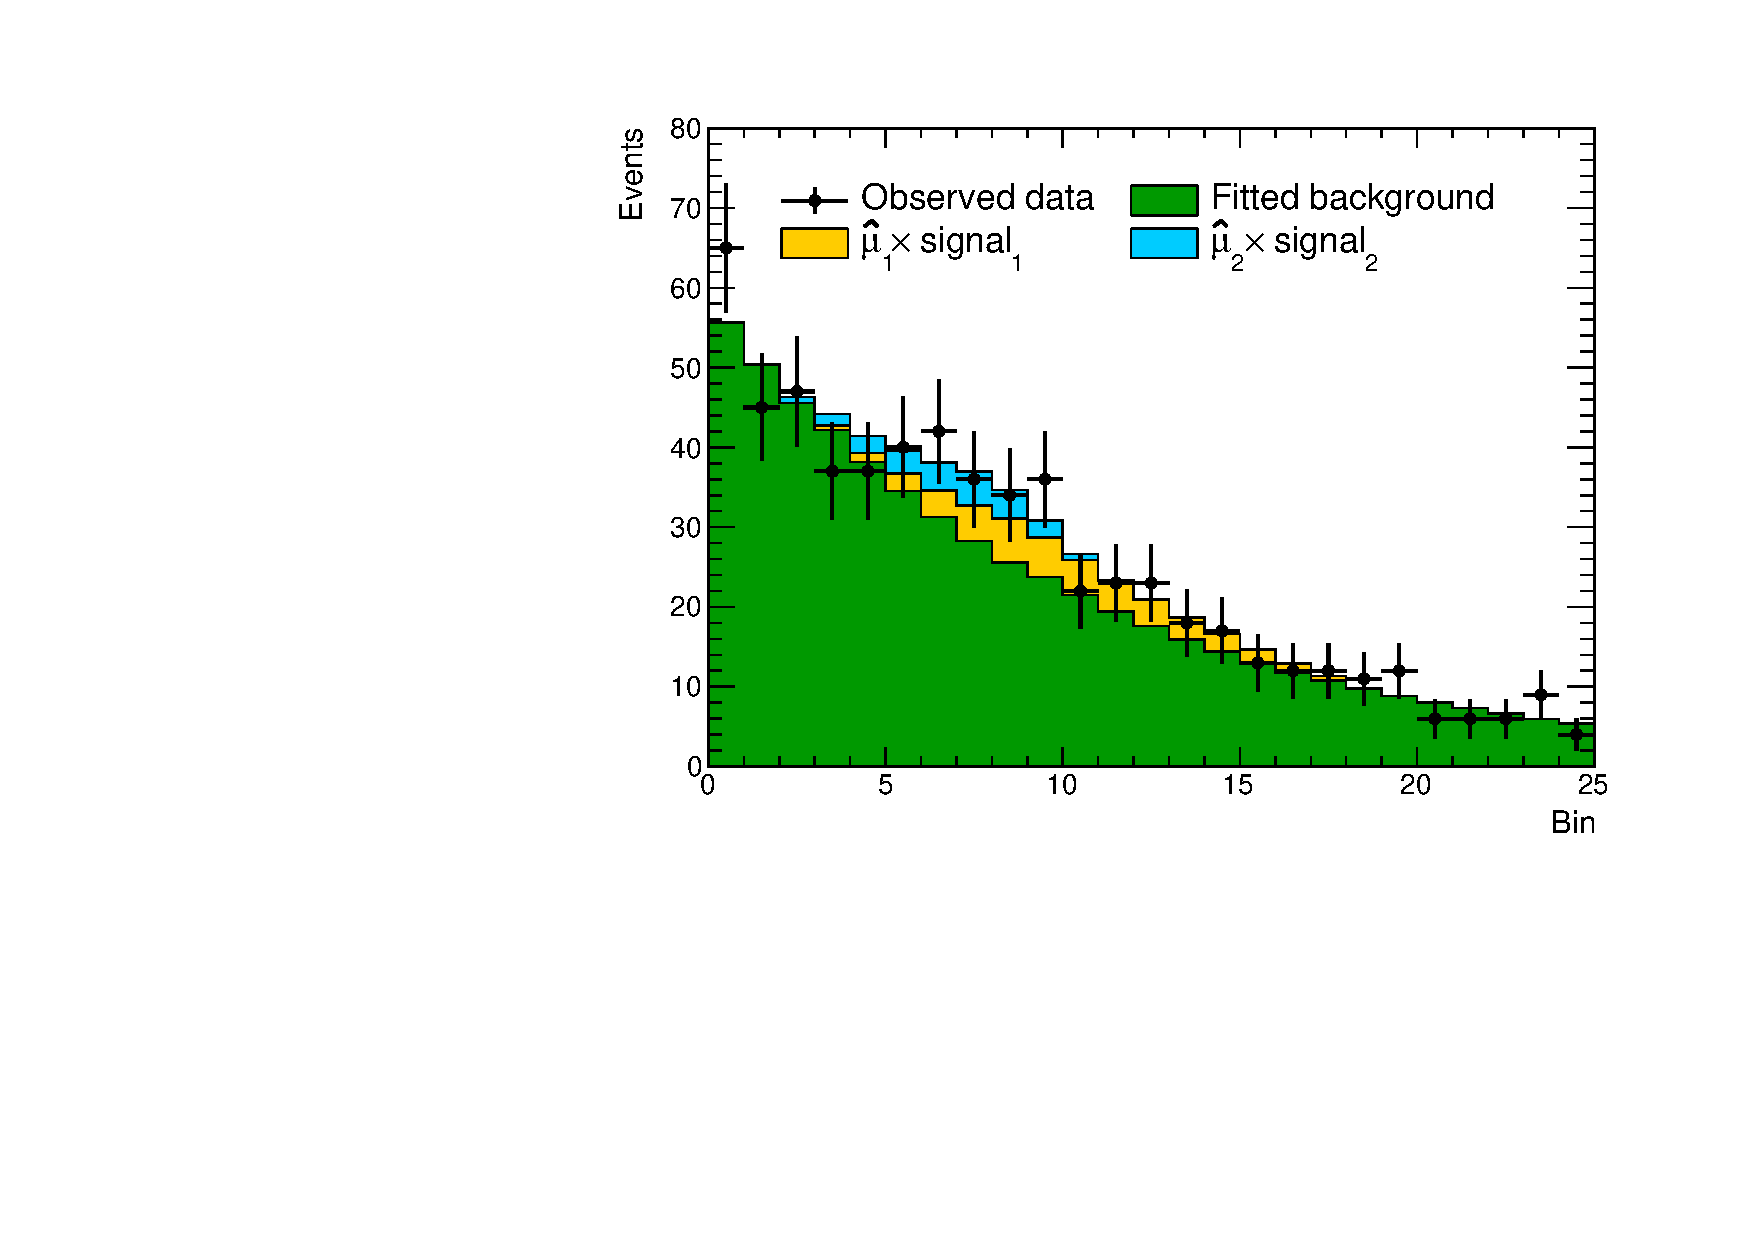
\includegraphics[width=0.8\textwidth]{figures/Intervals/data_model_plot.pdf}
    \caption{Background and signal distributions at the global minimum of the likelihood parameters, stacked on top of one another. The data is shown too, and the error bars represent the standard deviation of a Poisson with the same mean. }
    \label{fig:example_binneddata}
\end{figure}

\begin{figure}[hbt!]
    \centering
    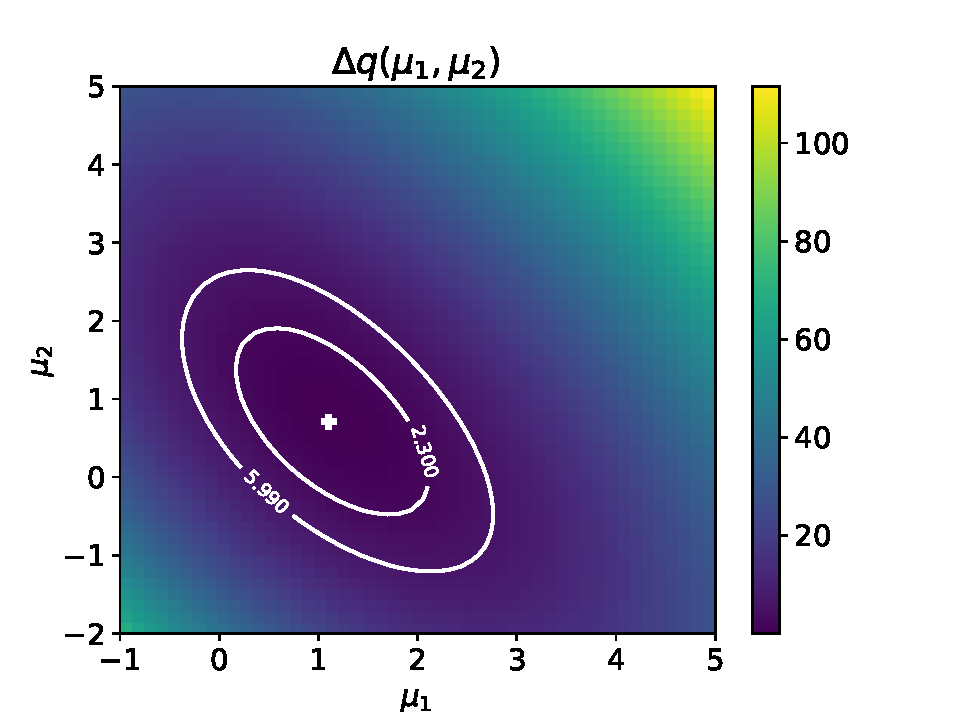
\includegraphics[width=0.49\textwidth]{figures/Intervals/likelihood_scan_mu1_mu2.pdf}
    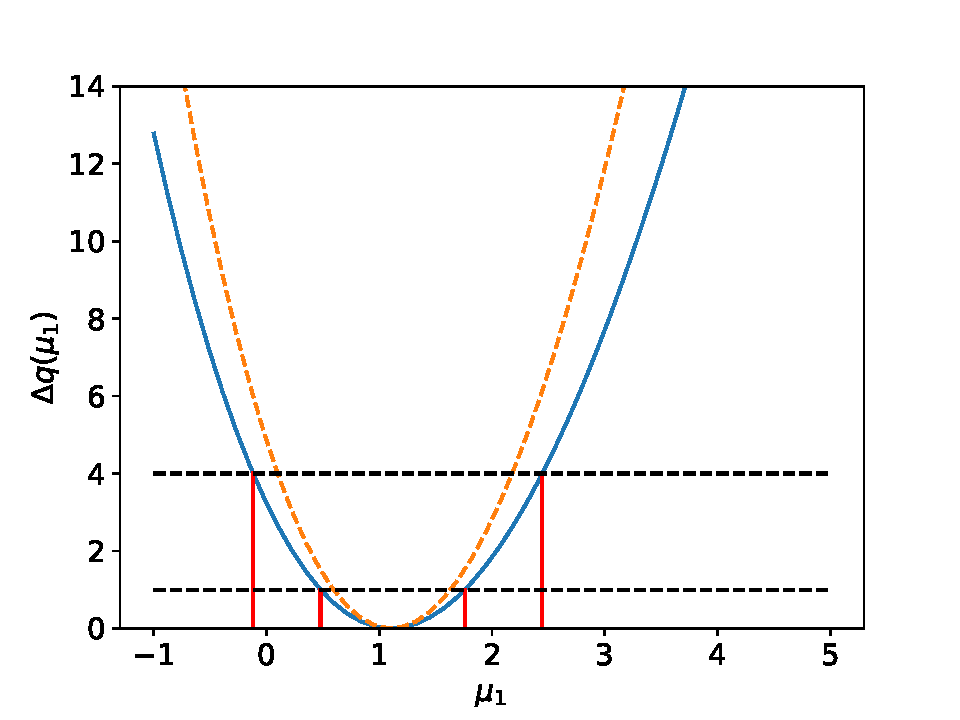
\includegraphics[width=0.49\textwidth]{figures/Intervals/scan_mu1.pdf}
    \caption{Left: $\Delta q(\mu_1,\mu_2)$ in color scale and contours corresponding to the boundaries of the 68.3\% and 95.4\% confidence regions. Right: $\Delta q(\mu_1)$ both profiling (blue line) and fixing $\mu_{2}$ (orange dashed line) the 68.3\% and 95.4\% confidence intervals are indicated by the red lines.   }
    \label{fig:example_binnedlh}
\end{figure}
Extracting the intervals/regions this way (using the profiled log-likelihood) is often referred to as the \textsf{MINOS} method (as this is the method used in the  \textsf{MINOS} code to determine uncertainties). 
 
Remember that in our definition of $\zeta_{\mu}$ for the simple counting experiment, we had two clauses depending on whether or not the signal strength ($\mu$) was greater than 0 or not. The introduction of this boundary poses no problem when constructing the frequentist intervals, however, it will have an effect when appealing to Wilks' theorem, as the assumption that $\zeta_{\mu}$ is distributed as a $\chi^{2}(2)$ will breakdown when $\mu\sim 0$. Figure~\ref{fig:example_fc} shows an example of this happening in a CMS analysis of Higgs boson decays to $\gamma\gamma$ with the Run-1 dataset. The parameters $\mu_{\mathrm{ggH+ttH}}$ and  $\mu_{\mathrm{VH+qqH}}$ are signal strengths for Higgs boson production modes involving fermion and vector-boson couplings, respectively. In this model, these parameters are bounded to be $>0$. The contours indicate the 68\% and 95\% confidence regions determined from the observed data using a Neyman construction with likelihood ratio ordering (labelled ``Feldman-Cousins'') and appealing to Wilks' theorem (labelled ``Likelihood Scan''). Away from the boundaries, the contours agree rather well -- meaning that the conditions for Wilks' theorem to apply hold. However, close to the boundaries, the contours start to disagree. This is not due to there being not enough events in the sample, but really a consequence of the boundary. It is therefore important to check the coverage of the intervals/regions reported when using the \textsf{MINOS} method, when there are boundaries in the problem. 
\begin{figure}[hbt!]
    \centering
    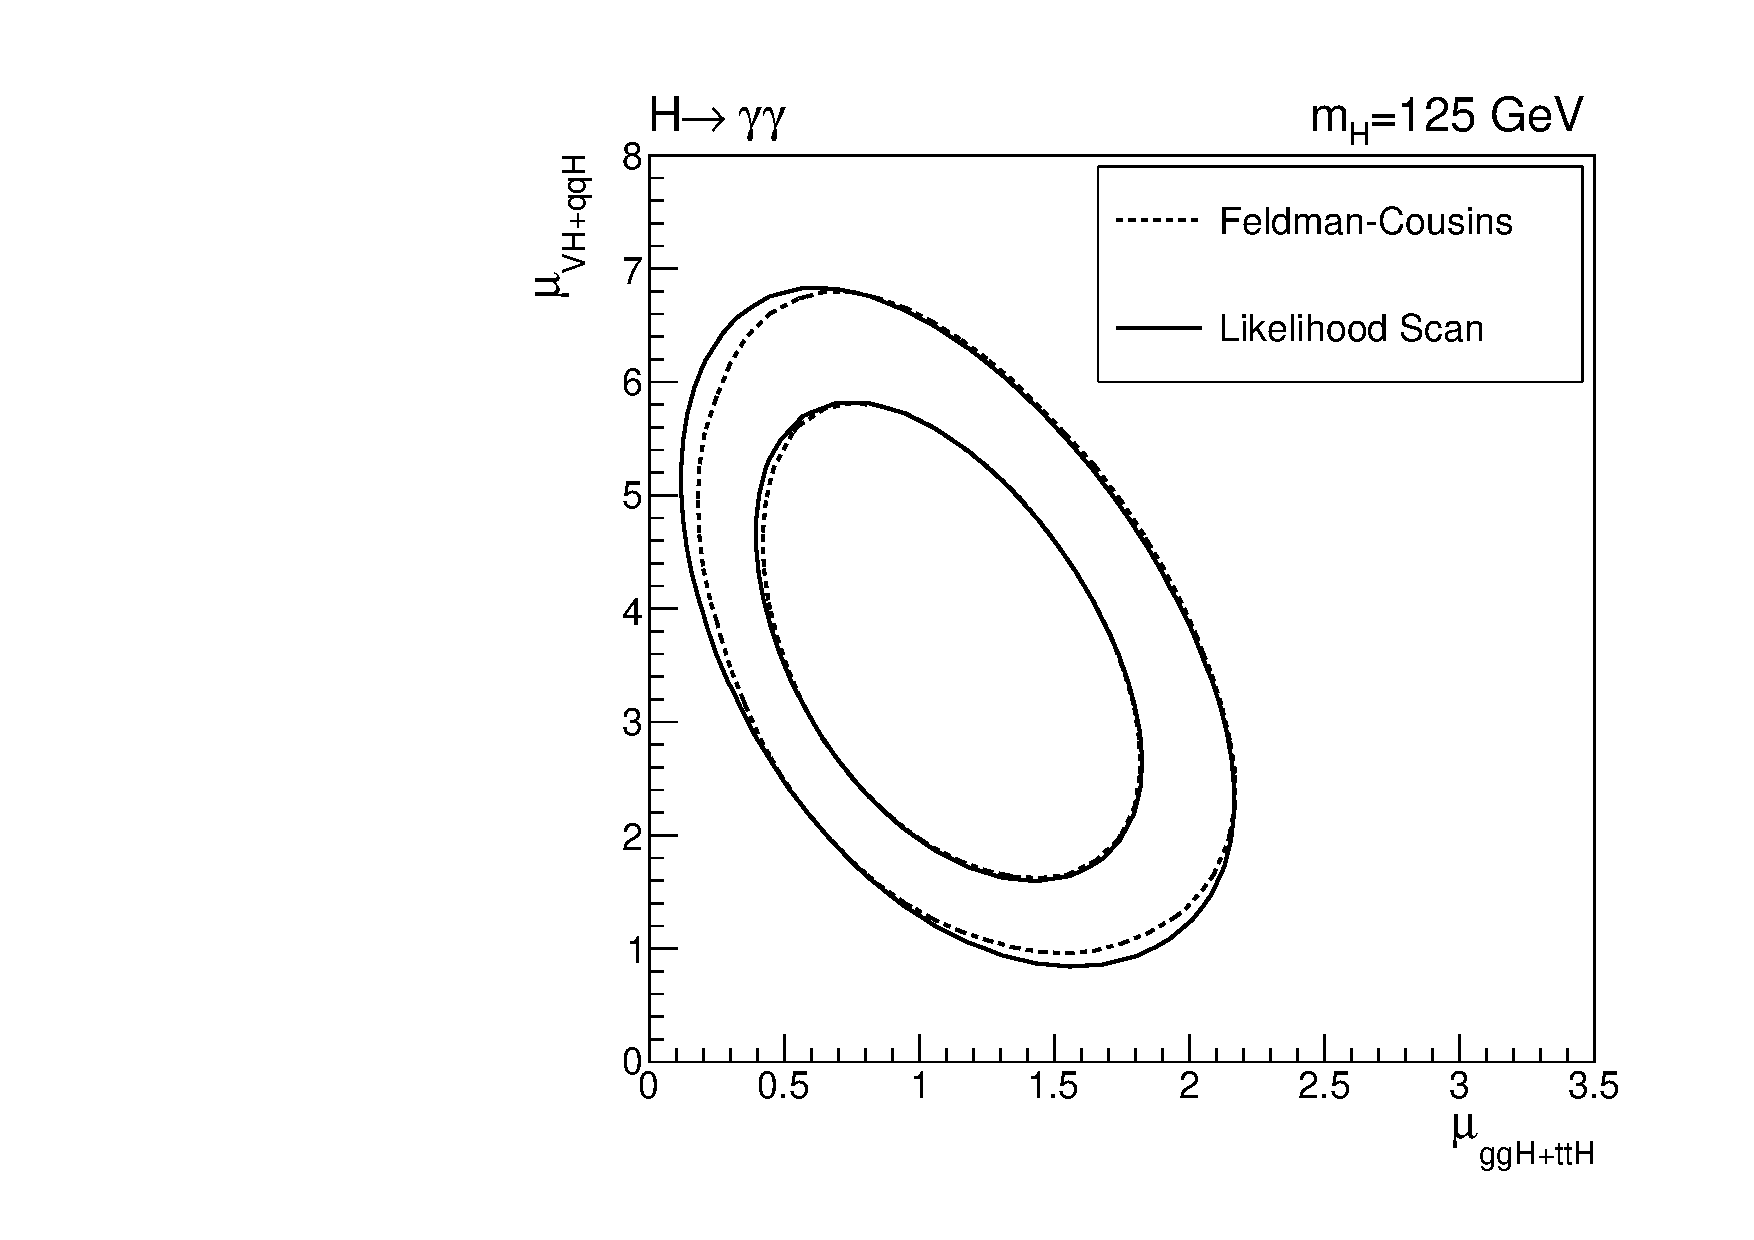
\includegraphics[width=0.6\textwidth]{figures/Intervals/compare-fc-lh.pdf}
    \caption{CMS analysis of Higgs boson decays to $\gamma\gamma$ with the Run-1 dataset. The two parameters are bounded to be $>0$. The contours indicate the 68\% and 95\% confidence regions determined from the observed data using a Neyman construction with likelihood ratio ordering (labelled ``Feldman-Cousins'') and appealing to Wilks' theorem (labelled ``Likelihood Scan'').}
    \label{fig:example_fc}
\end{figure}

\textcolor{red}{Add here something about the Hessian approach for approximating uncertainties, since this thing is gaussian near the minimum.}

Note that we can even go one step further in approximation. Let's go back to equation~\ref{eqn:taylor_exp_qN}. We can see that in 1-dimension, this is just a parabolic function. Re-arranging gives us the usual approximation,

\begin{equation}\label{eqn:hessianderive1d}
    2(q_{N}(\theta)-q(\hat{\theta})) = q''_{N}(\hat{\theta})(\theta-\hat{\theta})^{2}
\end{equation}

i.e twice the difference in the negative log-likelihood to the value at the minimum looks like a parabola, close to the minimum, that is centered at $\hat{\theta}$. If we had a random variable that was distributed as a Gaussian with $\theta\sim \phi(\hat{\theta},\sigma)$, we would find that that the twice the negative log-likelihood would be, 

\begin{equation}
-2\left(\ln(\phi(\theta,\sigma)) - \ln(\phi(\hat{\theta},\sigma)) \right)
= -2\left( \frac{1}{2}\left(\frac{\theta-\hat{\theta}}{\sigma}\right)^{2} - \frac{1}{2}\left(\frac{\hat{\theta}-\hat{\theta}}{\sigma}\right)^2\right)  
= \left(\frac{\theta-\hat{\theta}}{\sigma}\right)^{2},
\end{equation}

where constant terms cancel in the second step. This means if we match with equation~\ref{eqn:hessianderive1d}, we can clearly see that,

\begin{equation}
\frac{1}{\sigma^{2}} = q''_{N}(\hat{\theta}).
\end{equation}

So in this approximation, since for a Gaussian distribution, the 68.3\% interval is given by the standard deviation, our 68.3\% is given by the 2nd derivative of twice the difference in the negative log-likelihood function, evaluated at the minimum. This result extends to more than one dimension simply replacing $q''_{N}$ with the Hessian yields an approximation of the  co-variance matrix in multi-dimensional fits. However, often its better to use the method previously described finding the intervals via the crossings at set levels to determine confidence intervals, so we won't use this method further.  

\subsection{Coverage in the counting experiment}

Now let's return to our simple counting experiment. Close to the boundary $\mu=0$, we have two issues with applying Wilks' theorem. The first is not being in the limit of large $N$ and the second being the boundary itself. We can check what the coverage of the method (say for the 68.3\% interval) by determining the \emph{fraction of intervals} in $\mu$, as a function of the true value $\mu_0$, that contain $\mu_{0}$. It sounds like a rather painful ordeal given that calculating a single interval can take time, however, we do not need to calculate each interval to figure out the coverage. Remember that $\mu$ is included in the interval provided $\zeta^{\mathrm{obs}}_{\mu}\leq\zeta^{68.3}_{\mu}$. For the Neyman construction, we can use toys to calculate $\zeta^{68.3}_{\mu}$, while for the \textsf{MINOS} method, we assume $\zeta^{68.3}_{\mu}=1$. Figure~\ref{fig:coverage} shows the coverage in $\mu$ when calculating the intervals using the Neyman construction and using the \textsf{MINOS} method for our counting experiment.  
\begin{figure}[hbt!]
    \centering
    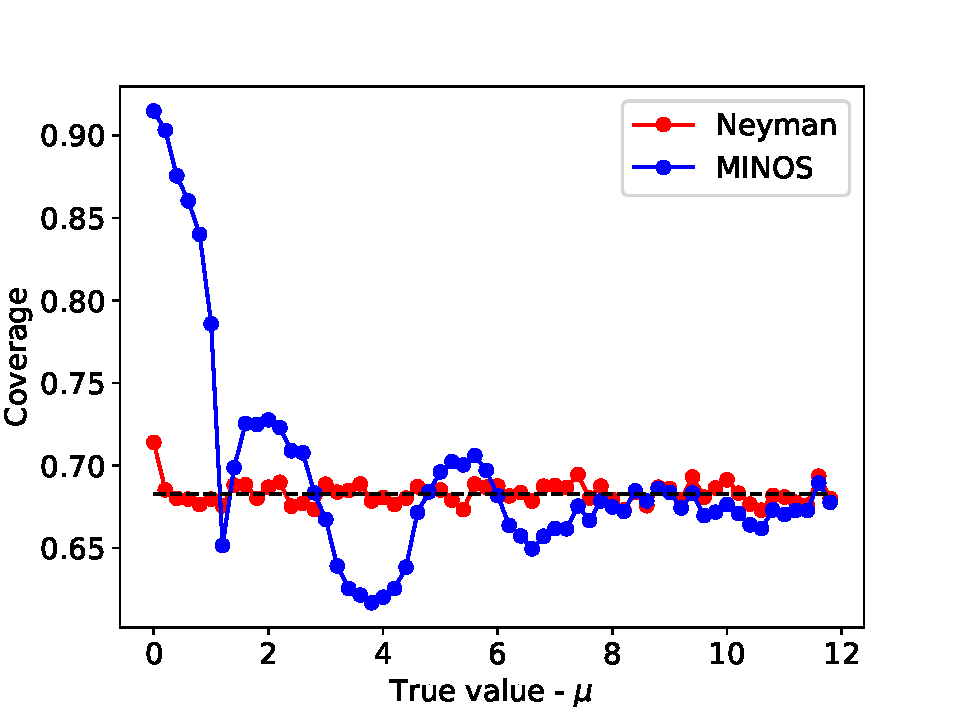
\includegraphics{figures/Intervals/coverage_example.pdf}
    \caption{Coverage of intervals in $\mu$ for the counting experiment, when calculated using the Neyman construction compared to the \textsf{MINOS} method, as a function of the true value $\mu$.}
    \label{fig:coverage}
\end{figure}
You can see that the Neyman construction gives very close coverage to the desired 68.3\% except at very small $\mu$, where the discrete nature of the Poisson distribution makes it difficult to find the exact $\zeta^{68.3}_{\mu}$ -- in fact this is still seen at larger values, though the effect gets reduced. Instead, the \textsf{MINOS} method, jumps between over-coverage and undercoverage, eventually settling down only above $\mu\sim 8$. This is not surprising since the distribution of $\zeta_{\mu}$ really doesn't look like a $\chi^{2}(1)$. Figure~\ref{fig:chisquare_zetamu} shows the distribution of $\zeta_{\mu}$ at $\mu=0.1$ and $\mu=9$. For the larger value, away from the boundary the approximation of a $\chi^{2}(1)$ is much more accurate. 
\begin{figure}
    \centering
    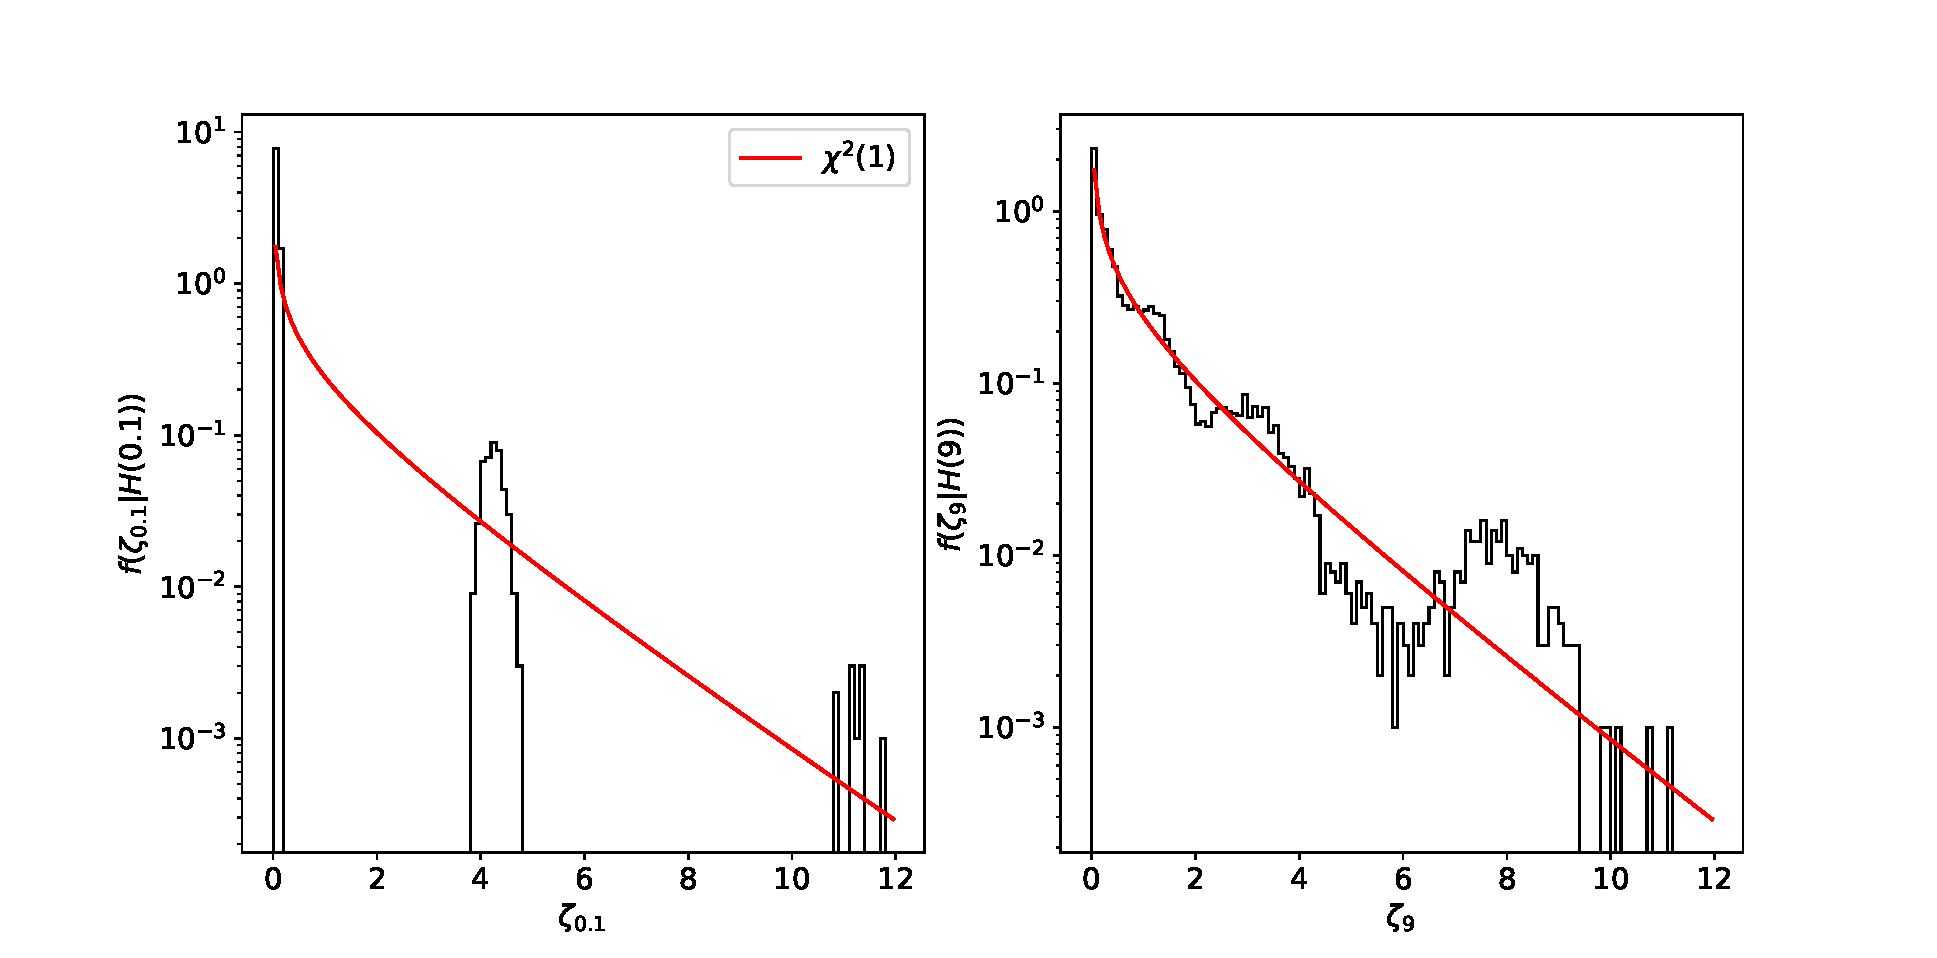
\includegraphics[width=\textwidth]{figures/Intervals/tmu_dists_example.pdf}
    \caption{Distribution of $\zeta_{\mu}$ for $\mu=0.1$ (left) and $\mu=9$, for the counting experiment, with a boundary $\mu>0$. The black histograms are the real distribution, evaluated using toys, while the red like is the approximate distribution using Wilks' theorem.}
    \label{fig:chisquare_zetamu}
\end{figure}

\subsection{Conversions to Z-scores}
The $\chi^{2}$ distribution is often used to provide a simple conversion from $p$-values (which can get very small) to more reasonable numbers. In HEP, you'll find that physicists thend to convert an observed $p$-value ($p$) into an equivalent ``\emph{number of sigma'' $n(\sigma)$} or Z-score for a normal distribution using, 
\begin{eqnarray}
    p & = &  \int_{Q}^{+\infty}\chi^{2}(X;1)dX \\
    \mathrm{Z}& = & \sqrt{Q}
\end{eqnarray} 
It should be noted that this is \emph{only a conversion convention} and doesn't tell us anything about the underlying distributions or the number of degrees of freedom. The conversion is always done using a $\chi^{2}(1)$. Eg, when a particle physicist talks about ``a more than 3$\sigma$ discrepancy'', they always mean that the $p-$value of the test under the null is smaller than $\int_{3^{2}}^{\infty}\chi^{2}(X;1)dX$. 

Often, particle physicists will refer to a \emph{1-sided} test, in which case the conversion is performed using the following, 
\begin{eqnarray}\label{eqn:convertpval}
    p & = & \int_{Q}^{+\infty}\left(\frac{1}{2}\delta(0)+\frac{1}{2}\chi^{2}(X;1)\right)dX \\
    \mathrm{Z}& = & \sqrt{Q}
\end{eqnarray} 
Usually this is the case when talking about ``discovery'' of a new process. For example, the test statistic used in the Higgs boson discovery (and in many results since), was, 
\begin{equation}
    t_{0} = \begin{cases}
                q(0,\hat{\eta}_{0})-q(\hat{\mu},\hat{\eta})    & \hat{\mu} > 0 \\
                0               & \hat{\mu}\leq 0,
                \end{cases}
\end{equation}
where $\mu$ is an overall signal rate multiplier, and we are interested in rejecting the hypothesis $\mu=0$ -- $H(0)$. It can be shown that in the limit of large numbers, $f(t_{0}|H(0)) = \frac{1}{2}\delta(0)+\frac{1}{2}\chi^{2}(t_0;1)$, meaning the $p$-value ($p_{0})$ can be calculated using Eqn~\ref{eqn:convertpval}, and the Z-score is $\sqrt{t^{\mathrm{obs}}_{0}}$. Particle physicists get excited when $t_{0}^{\mathrm{obs}}>25$ -- which corresponds to the ``5 sigma discovery''. I personally think this all adds more confusion than clarification and the best practise is to explain the hypotheses being performed and the criteria to reject or accept hypotheses. 

\subsection{Bayesian credible intervals}
As a last remark, we should return to the Bayesian's answer for what $X\pm\sigma_{X}$ means. It's a lot more simple than the freqeuntist answer, but remember that the interpretation is quite different. Once the posterior distribution $P(\mu)$ is obtained (by marginalising over the nuisance parameters $\eta$, a Bayesian can quote a $(100\times\alpha)$\% \emph{credible interval} (or credible region in more than one dimension), as a region $\mu\in\Omega_{\alpha}$ for which,
\begin{equation}\label{eqn:credible}
    P(\mu\in\Omega_{\alpha})=\int_{\Omega_{\alpha}} P(\mu)d\mu = \alpha.
\end{equation}
Its as simple as that right? Not quite! There can be multiple such regions, any of which satisfy Eqn.~\ref{eqn:credible}. It's best to show the posterior distribution in publications, and describe any interval that is quoted as a result. Below is a snippet of python code that calculates the \emph{shortest} 68.3\% interval for our countin experiment. Note that many of the functions were already defined in Section~\ref{sec:marginalised}, so I won't bother repeating them.
\begin{lstlisting}[style = Python]
import marginalised_likelihood

# new prior on mu P(mu)
def prior_mu_new(mu):
  if (mu > 50 or mu < 0) : return 0
  else: return 1./50

marginalised_likelihood.prior_mu = prior_mu_new

marginalised_likelihood.prior_mu = prior_mu_new
xaxis = numpy.linspace(-1,20,5000)
normalisation = marginalised_likelihood.norm(n)
posterior_dist = [ marginalised_likelihood.integral(n,mu)/normalisation \
for mu in xaxis ]

# use an approximate for the integral with rectangles
intervals=[]
for i in range(len(xaxis)):
 x = xaxis[i]
 if x > 5: break
 inte=0
 for j in range(i,len(xaxis)-1):
   y = xaxis[j+1]
   yl = xaxis[j]
   inte += posterior_dist[j]*(y-yl)
   if inte >= 0.683:
    intervals.append([y-x,[x,y],[i,j]])
    break

# find the shortest one
intervals.sort(); interval = intervals[0]
print("68.3%% interval (%.2f,%.2f)"%(interval[1][0],interval[1][1]))
\end{lstlisting}

Figure~\ref{fig:posterior_shortest_interval} shows the posterior distribution $P(\mu)$ for the counting experiment, this time restricting $\mu>0$ by setting the prior $\pi(\mu)=0$ for $\mu\leq0$. The shaded region indicates the shortest 68.3\% credible interval for $\mu$. 

\begin{figure}[hbt!]
    \centering
    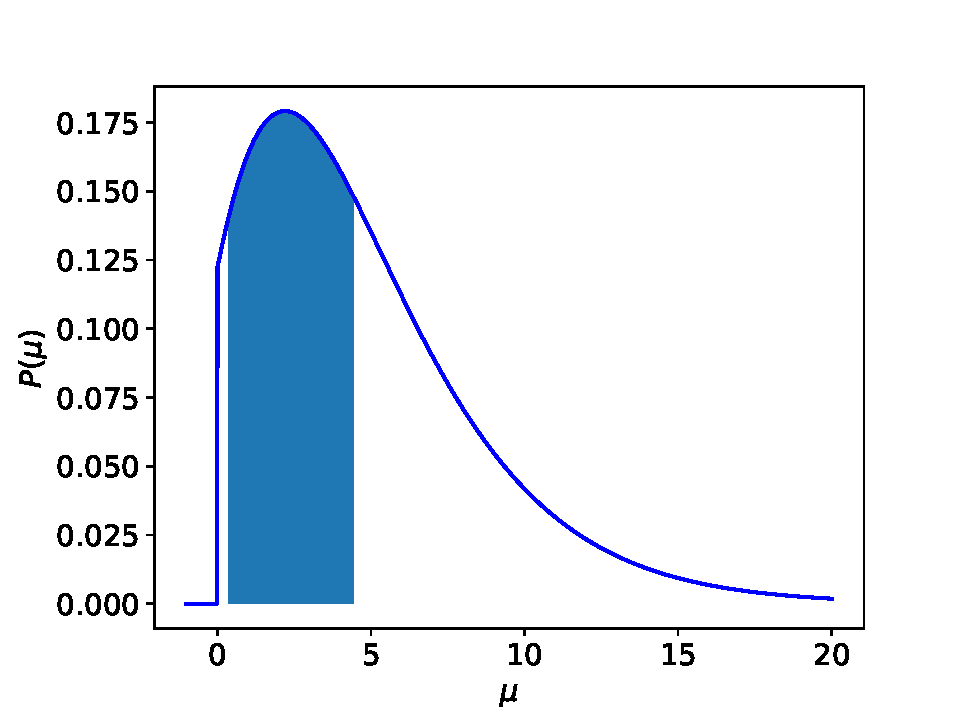
\includegraphics[width=0.8\textwidth]{figures/Intervals/credible_interval.pdf}
    \caption{Posterior $P(\mu)$ for the counting experiment, restricting $\mu>0$ in the prior for $\mu$. The shaded region indicates the shortest 68.3\% credible region.  }
    \label{fig:posterior_shortest_interval}
\end{figure}

In addition to choosing an interval, as always, studying the effect of changing priors $\pi(\mu)$ is a must for Bayesian credible intervals. So long as the data is powerful enough, $P(\mu)$ should be fairly insensitive to this choice -- but its not guaranteed! 